\documentclass[12pt,aspectratio=169]{beamer}
% \hypersetup{pdfpagemode=FullScreen}

\usepackage{upgreek}
\usefonttheme{professionalfonts}

\renewcommand*{\thefootnote}{\fnsymbol{footnote}}

\mode<presentation>
\useoutertheme[subsection=false]{miniframes}

\title{Outrageously Large Neural Networks: The Sparsely-Gated Mixture-of-Experts Layer}
\author{Noam Shazeer\inst{1} \and Azalia Mirhoseini\inst{1} \and Krzysztof Maziarz\inst{2} \and Andy Davis\inst{1} \and Quoc Le\inst{1} \and Geoffrey Hinton\inst{1} \and Jeff Dean\inst{1}}
\institute{\inst{1} Google Brain
           \inst{2} Jagiellonian University, Cracow}
\date{ICLR 2017}

\begin{document}
    \beamertemplatenavigationsymbolsempty

    \makeatletter
    \def\beamer@andinst{\\[.1em]}
    \makeatother

    \begin{frame}
        \titlepage
    \end{frame}

    \section{Introduction}

    \begin{frame}
        \frametitle{Background}

        \begin{itemize}
            \setlength{\itemsep}{.8em}
            \item Practices in various domains including text, images, and audio have shown that with sufficiently large datasets, increasing the capacity (number of parameters) of neural networks can give much better prediction accuracy.
            \item For typical deep learning models, where the entire model is activated for every example, the training costs are quadratic, as both the model size and the number of training examples increase.
        \end{itemize}
    \end{frame}

    \begin{frame}
        \frametitle{Motivation}

        \begin{itemize}
            \setlength{\itemsep}{.8em}
            \item Various forms of conditional computation have been proposed as a way to increase model capacity without a proportional increase in computational costs.
            \item In these schemes, large parts of a network are active or inactive on a per-example basis.
            \item However, While these ideas are promising in theory, no work to date has yet demonstrated massive improvements in model capacity, training time, or model quality.
        \end{itemize}
    \end{frame}

    \begin{frame}
        \frametitle{Challenges}

        \begin{itemize}
            \setlength{\itemsep}{.8em}
            \item GPUs are much faster at arithmetic than at branching.
            \item Conditional computation reduces the batch sizes for the conditionally active chunks, resulting in lower GPU utilization.
            \item Network bandwidth could be more limiting than computation power.
            \item Additional loss terms may be necessary to achieve the desired level of sparsity.
            \item Model capacity is most critical for very large datasets. Previous studies use datasets up to 600,000 images, which may not be able to demonstrate the necessity of huge models.
        \end{itemize}
    \end{frame}

    \section{Method}

    \begin{frame}
        \frametitle{Sparsely-Gated Mixture-of-Experts (MoE) Layers}

        \begin{columns}
        \begin{column}{0.35\textwidth}
            A new type of general purpose neural network componenet, Sparsely-Gated Mixture-of-Experts (MoE) Layer,
            which consists of a number of experts, each a simple feed-forward neural network, and a trainable gating network.
        \end{column}
        \begin{column}{0.65\textwidth}
            \includegraphics[page=2,trim=4cm 18.7cm 5.2cm 3cm,clip,scale=0.73]{MoE.pdf}
        \end{column}
        \end{columns}
    \end{frame}

    \begin{frame}
        \frametitle{Sparsely-Gated Mixture-of-Experts (MoE) Layers}

        $$ y = \sum^n_{i=1}G(x)_iE_i(x) $$

        $G(x)$ is the gating network. Wherever $G(x)_i = 0$, the computation of $E_i(x)$ can be skipped.

        $E_i(x)$ is the output of the i-th expert.

    \end{frame}

    \begin{frame}
        \frametitle{Gating Network}

        \begin{itemize}
            \setlength{\itemsep}{.8em}
            \item A simple choice (Jordan et al., 1994) is $G(x) = Softmax(x \cdot W_g)$
            \item However, to achieve sparsity, a new Noisy Top-K Gating is introduced.
        \end{itemize}

        \vskip -.8em
        $$ G(x) = Softmax(KeepTopK(H(x), k) $$
        $$ H(x)_i = (x \cdot W_g)_i + StandardNormal() \cdot Softplus((x \cdot W_{noise})_i) $$
        $$ KeepTopK(v, k)_i = \begin{cases}
            v_i & \text{if $v_i$ is in the top $k$ elements of $v$}\\
            -\infty & \text{otherwise}\\
          \end{cases} $$

        \begin{itemize}
            \item The gating network can be trained with back-propagation.
        \end{itemize}
    \end{frame}

    \section{Implementation}

    \begin{frame}
        \frametitle{The Shrinking Batch Problem}

        Large batch sizes are necessary for computation efficiency on mordern GPUs. If the gating network chooses $k$
        out of $n$ experts, then for a batch of $b$ examples, each experts receives approximately $\frac{kb}{n} \ll b$
        examples.

        \vskip 1em

        The solution is to make the original batch size as large as possible. However, batch size tends to be limited by
        the memory necessary to store activations between the forwards and backwards passes.
    \end{frame}

    \begin{frame}
        \frametitle{Mixing Data Parallelism and Model Parallelism}

        \begin{columns}
        \begin{column}{0.55\textwidth}
            \begin{itemize}
                \setlength{\itemsep}{.8em}
                \item Distribute the standard layers and the gating networks according to conventional data-parallel schemes, allowing large total batch size.
                \item Each expert in the MoE layer receives a combined batch consisting of the relevant examples from all of the data-parallel input batches.
            \end{itemize}
        \end{column}
        \begin{column}{0.45\textwidth}
            \centering
            \includegraphics[page=5,trim=10.5cm 16.8cm 4cm 3cm,clip,scale=0.8]{GShards.pdf}
        \end{column}
        \end{columns}
    \end{frame}

    \begin{frame}
        \frametitle{Taking Advantage of Convolutionality}

        In the language model used in the experiment, another trick to the shrinking batch size problem is to accumulate
        the data of all the time steps of the previous layer as a big batch before feeding into the MoE layer. This is
        because the MoE layer is not recurrent and is applied to all the time steps convolutionally.
    \end{frame}

    \begin{frame}
        \frametitle{Network Bandwidth}

        \begin{itemize}
            \setlength{\itemsep}{.8em}
            \item Sending the inputs and outputs of the experts across the network takes significant time.
            \item To maintain computational efficiency, the hidden layer of each expert can be set to very big, or more hidden layers can be used.
        \end{itemize}
    \end{frame}

    \begin{frame}
        \frametitle{Balancing Experts Utilization}

        \begin{itemize}
            \setlength{\itemsep}{.8em}
            \item Imbalanced choice of experts wastes capacity and slows down training.
            \item The imbalance of gating network is self-reinforcing, as the favored experts are trained more rapidly.
            \item Therefore, an importance loss is introduced to encourage all experts to have equal importance.
        \end{itemize}

        $$ Importance(X) = \sum_{x \in X}G(x) $$
        $$ L_{importance}(X) = \lambda \cdot CV(Importance(X))^2 $$
    \end{frame}

    \section{Experiments}

    \begin{frame}
        \frametitle{1 Billion Word Language Modeling Benchmark}

        \begin{itemize}
            \setlength{\itemsep}{.8em}
            \item Dataset: shuffled sentences that have approximately 829 million words with a vocabulary of 793,471 words.
            \item Baseline: one or more stacked LSTM layers.
            \item MoE model: two stacked LSTM with a MoE layer between. 4 experts were active per input.
        \end{itemize}
    \end{frame}

    \begin{frame}
        \frametitle{Low Computation, Varied Capacity}

        The first experiment shows the effect of adding capacity while keeping the computation cost roughly the same.

        \centering
        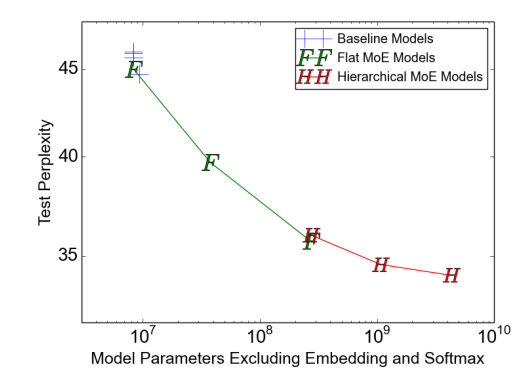
\includegraphics[scale=0.35]{exp1.png}
    \end{frame}

    \begin{frame}
        \frametitle{Varied Computation, High Capacity}

        The next experiment alters the number of experts and the width of each expert, to adjust the computation cost while
        keeping the capacity the same.

        \vskip 0.5em
        \centering
        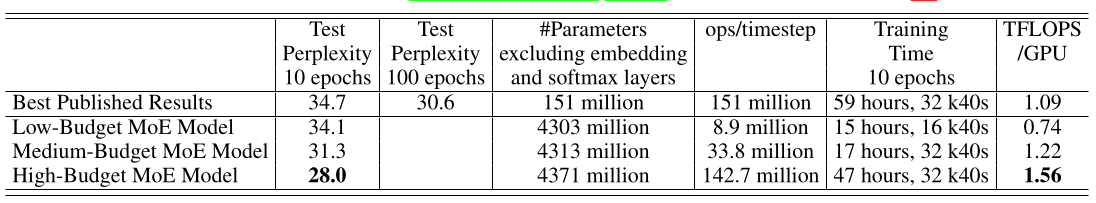
\includegraphics[scale=0.35]{exp2.png}
    \end{frame}

    \begin{frame}
        \frametitle{Machine Translation}

        The MoE model is modified from the GNMT model. It shows better performance in the WMT'14 English to Franch
        translation task with lower computation cost.

        \vskip 0.5em
        \centering
        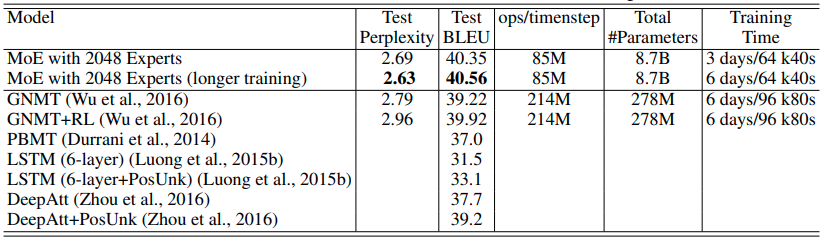
\includegraphics[scale=0.45]{exp3.png}
    \end{frame}

    \begin{frame}
        \frametitle{Multilingual Machine Translation}

        \centering
        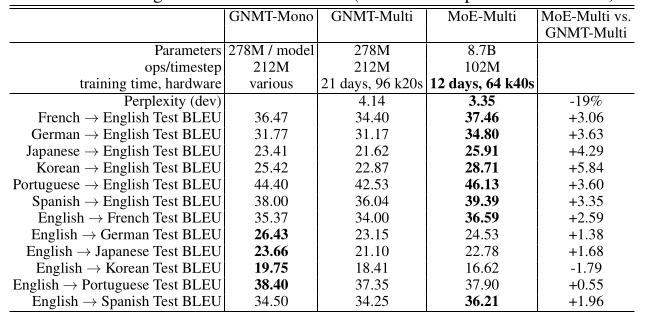
\includegraphics[scale=0.45]{exp4.png}
    \end{frame}

    \appendix

    \begin{frame}
        \frametitle{Conclusion}

        The paper presented a conditional computation layer and showed its power in increasing the model capacity
        without quadratic computation cost. It also introduces new engineering challenges like shrinking batchsize
        problem and expert imbalance. There are follow up papers like GShard in ICLR 2021 that further investigate these
        problems. We can also think about them and try to find better solutions.
    \end{frame}

    \begin{frame}
        \vskip 1.5em

        \centering \huge
        Thank you!
    \end{frame}
\end{document}
